\documentclass[../main.tex]{subfiles}
\graphicspath{
    {"../img/"}
    {"img/"}
}

\begin{document}
    Weźmy takie równanie różniczkowe
    \[
        U_{,t} + c U_{,x} = 0
    .\]
Ustawiamy $U$ takie o
\[
    U(t,x): \left]0,\infty\right[ \times \mathbb{R} \to \mathbb{R},\quad U(0,x) = U_0(x)
.\]

\[
    \left[ U_{,t}, U_{,x} \right] \begin{bmatrix} 1\\c \end{bmatrix} = 0
.\]
Ciekawi nas, czy istnieje taka parametryzacja $(t(s), x(t))$, że rozwiązanie $U$ jest na niej stałe? Czyli
\[
    \frac{d}{ds} U(t(s), x(s)) = 0
.\]
Spróbujmy tak
\[
    \frac{\partial x}{\partial s} = c,\quad \frac{\partial t}{\partial s} = 1
.\]
Wtedy $x = c s + x_0$, $t = s + t_0$
Jeżeli $t = 0, s = 0$, to $t_0 = 0$.\\
Czyli mamy
\[
    \begin{cases}
        x = cs + x_0\\
        t = s
    \end{cases} \implies x = ct + x_0 \implies x_0 = x - ct
.\]
No to teraz
\[
    U(x,t) - U_0(x_0) = U_0(x-ct)
.\]

(Sprawdzić czy przypadkiem czegoś podobnego nie było na mechanice klasycznej pod folderem Równania Hamiltona-Jacobiego)

\begin{tw}
    (Równanie Burgersa)\\
    \[
        U_{,t} + U \cdot U_{,x} = 0,\quad U(0,x) = \phi(x)
    .\]
\[
    \phi(x) = \begin{cases}
        1 & x <0\\
        1-x & 0\le x \le 1\\
        0 &1 < x
    \end{cases}
.\]
\end{tw}

Rozważmy coś takiego
\[
    \left[ U_{,t}, U_{,x} \right] \begin{bmatrix} 1\\U \end{bmatrix} = 0
.\]
W parametryzacji $(x(s), t(s))$ - poziomica $U(t,x)$.
Czyli dla jakiegoś $z$
 \[
     U(t(s),x(s)) = z(s)
\]
jest stała.
\[
    \begin{cases}
        \frac{\partial t}{\partial s} = 1\\
        \frac{\partial x}{\partial s} = z(s)\\
        \frac{\partial z}{\partial s} = 0
    \end{cases}
.\]
Zakładamy warunki $t(0) = 0$, $x(0) = x_0$,
\[
    z(0) = U(t(0), x(0)) = U(0,x_0) = \phi(x_0)
.\]
Czyli skoro $z(s) = const$, to znaczy, że
 \[
     z(s) = \phi(x_0) \implies \begin{cases}
         \frac{\partial t}{\partial s} = 1\\
         \frac{\partial x}{\partial s} = \phi(x_0)\\
         \frac{\partial z}{\partial s} = \frac{\partial }{\partial s} \left( \phi(x_0) \right) = 0
     \end{cases}
.\]
Czyli tak
\[
    t = 1 \cdot s + t_0,\quad (t(0) = 0) \implies t = s
.\]
\[
    \begin{cases}
        x(s) = \phi(x_0) s + x_0\\
        z(s) = \phi(x_0)
    \end{cases}
.\]
Zmieniamy parametryzację, czyli
\[
    x(t) = \phi(x_0)t + x_0
.\]
\textit{Cała zabawa polega na tym, że mając punkt muszę umieć się cofnąć}. To jaki kształt ma charakterystyka, to nie ma za bardzo znaczenia, ale tak długo jak istnieje parametryzacja i można się cofnąć to jest ok.\\
Rysujemy linie, wzdłuż których nasze rozwiązanie jest stałe (rys \ref{fig:charakterystyki})
Dla $x_0 < 0$ mamy $x(t) = t + x_0$, i $x_0 > 1$ \\
Dla $0 < x_0 < 1$ mamy $x(t) = (1-x_0)t + x_0$, czyli to jakie dostajemy rozwiązanie to bardzo mocno zależy, od tego gdzie stoimy na początku

\begin{definicja}
    (Słabe rozwiązania)\\
    Niech $\mathcal{C}^1 \ni \varphi(t,x): \left]0, \infty\right[ \times \mathbb{R}\to \mathbb{R}$ ma zwarty nośnik.\\
    Mówimy, że
    \[
        U: \left]0,\infty\right[\times\mathbb{R}
    \]
    jest słabym rozwiązaniem równania
    \[
        U_{,t} + \left( F(U) \right)_{,x} = 0
    ,\]
jeżeli
\[
    \underset{\varphi}{\forall} \int\limits_{0}^{\infty} dt \int\limits_{-\infty}^{\infty} dx \left( U_{,t} + \left( F(U) \right)_{,x} \right) \varphi(x,t) = 0
.\]
\textbf{Uwaga: } te dwa warunki mają różne dziedziny!
\end{definicja}
\begin{figure}[h]
    \centering
    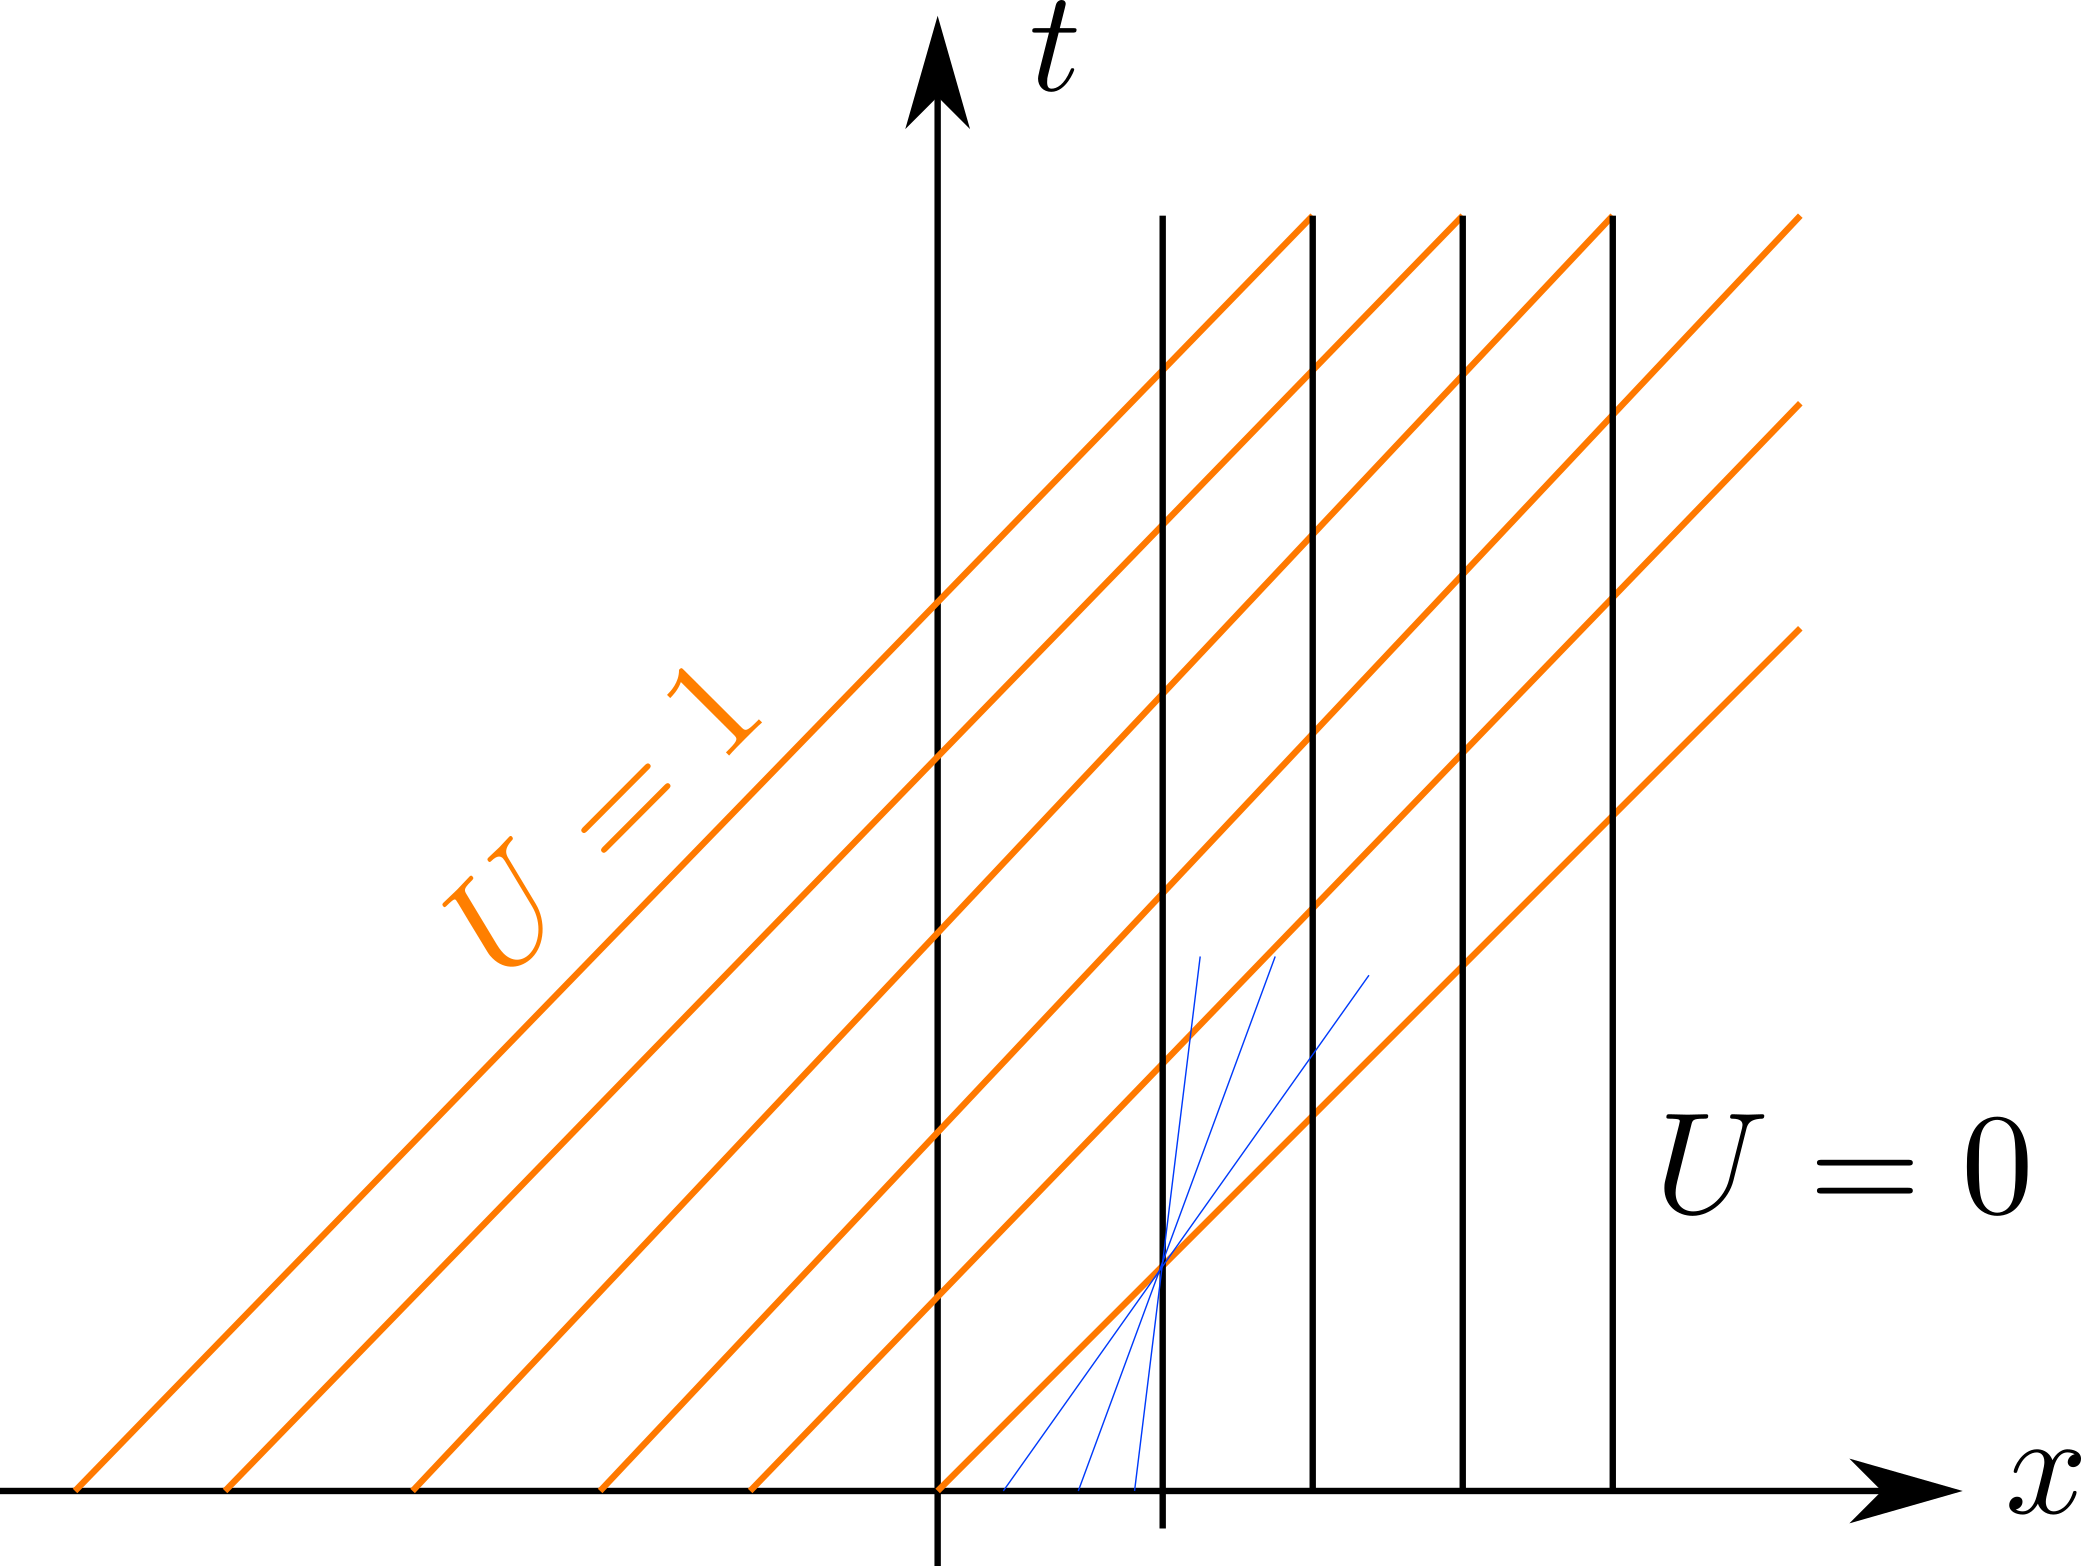
\includegraphics[width=0.8\textwidth]{charakterystyki}
    \caption{Jak wyglądają nasze charakterystyki?}
    \label{fig:charakterystyki}
\end{figure}

\[
    \int\limits_{-\infty}^{\infty} dx \int\limits_{0}^{\infty} dt U_{,t}\varphi(x,t) + \int\limits_{0}^{\infty} dt \int\limits_{-\infty}^{\infty} dx \left( F(U) \right)_{,x} \varphi(x,t)=
\]
Całkujemy przez części
\begin{align*}
    &= \int\limits_{-\infty}^{\infty} dx \left[ U \varphi(x,t) \right]_0^{+\infty} - \int\limits_{-\infty}^{\infty} dx \int\limits_{0}^{\infty} dt U(x,t)\varphi_{,t} +\\
    &+ \int\limits_{0}^{\infty} dt F(U)\varphi(x,t)_{-\infty}^{+\infty} - \int\limits_{0}^{\infty} dt \int\limits_{-\infty}^{\infty}dx  F(U)\varphi_{,x}
.\end{align*}
Przedostatnie się zeruje bo $\varphi$ ma nośnik zwarty, pierwsze do połowy wywalamy z tego samego powodu.
\[
    - \int\limits_{-\infty}^{\infty} dx \int\limits_{0}^{\infty} dt \left[ U\varphi_{,t}+F(U)\varphi_{,x} \right] - \int\limits_{-\infty}^{\infty} dx U(0, x)\varphi(x,0)
.\]

Czyli warunek z definicji jest w sensie słabych rozwiązań równoważny warunkowi
\[
    \underset{\varphi}{\forall} \int\limits_{-\infty}^{\infty} dx \int\limits_{0}^{\infty} dt \left[ U \varphi_{,t} + F(U) \varphi_{,x} \right] + \int\limits_{-\infty}^{\infty} dx g(x)\varphi(x,0) = 0
.\]
\begin{stw}
    (Przypomnienie)\\
    Niech $V\subset \left]0,\infty\right[\times\mathbb{R}$ - rozmaitość.\\
    Dla $\omega\in \Lambda^1(V)$ mamy
    \[
        \int\limits_{\partial V}\omega = \int\limits_V d\omega
    .\]
\[
    \int\limits_{\partial V}\star\omega = \int\limits_V d\left( \star \omega \right)
.\]
\end{stw}
Niech
\[
    A = A^{t + A^x dx}
,\]
wtedy \[
    d\star A = - \frac{\partial A^x}{\partial x} dx\land dt + \frac{\partial A^t}{\partial t} dt\land dx = \left( \frac{\partial A^t}{\partial t} + \frac{\partial A^x}{\partial x}  \right) dt\land dx
.\]
Podstawiając do tw. Stokesa
\[
    \int\limits_{V} \left( \frac{\partial A^t}{\partial t} + \frac{\partial A^x}{\partial x}  \right) dt\land dx = \int\limits_{\partial V}\left<-A^xdt + A^t dx, \frac{\partial }{\partial V}  \right>
.\]
Zakładamy, że brzeg $V$ możemy sparametryzować jakoś fajnie
\[
    \partial V = \left\{ \begin{bmatrix} c^t(s)\\c^x(s) \end{bmatrix} , s\in \left]0,1\right[ \right\}
.\]
Czyli
\[
    \frac{\partial }{\partial V} = \frac{\partial c^t}{\partial s} \frac{\partial }{\partial t} + \frac{\partial c^x}{\partial s} \frac{\partial }{\partial x}
.\]
Bierzemy RHS stokesa
\begin{align*}
    &\left<-A^xdt + A^t dx, \frac{\partial c^t}{\partial s} \frac{\partial }{\partial t} + \frac{\partial c^x}{\partial s} \frac{\partial }{\partial x}  \right> = -A^x \frac{\partial c^t}{\partial s} + A^t \frac{\partial c^x}{\partial s} = \\
    &= \left[ A^t, A^x \right] \begin{bmatrix} \frac{\partial c^x}{\partial s} \\ \frac{\partial c^t}{\partial s}  \end{bmatrix} = \\
        &= \mathbf{A} \cdot \mathbf{n}
\end{align*}
prostopadły do wektora stycznego. Czyli
\[
    \int\limits_V\left( \frac{\partial A^t}{\partial t} + \frac{\partial A^x}{\partial x}  \right) dV = \int\limits_{\partial V}\mathbf{A}\cdot \mathbf{n} \cdot \mathbf{dL}
.\]

\begin{stw}
    (Warunek Cauchy-Hugoniot)(Rankine-Hugoniot tak naprawdę)\\
    Szukamy krzywej, która pozwala na wybór wartości $U(x,t)$, w obszarze, w którym charakterystyki przecinają się.
\end{stw}
Wiemy, że na $V_I$ (\ref{fig:podzial_przestrzeni})
 \[
     U^I_{,t} + F\left( U^I_{,x} \right) = 0
.\]
Na $V_{II}$
 \[
     U^{II}_{,t} + F\left( U^{II} \right)_{,x} = 0
 .\]
 Szukamy funkcji $U$, która na $V$ jest słabym rozwiązaniem równania
 \[
     U_{,t} + F(U)_{,x} = 0
 .\]

 \begin{figure}[h]
     \centering
     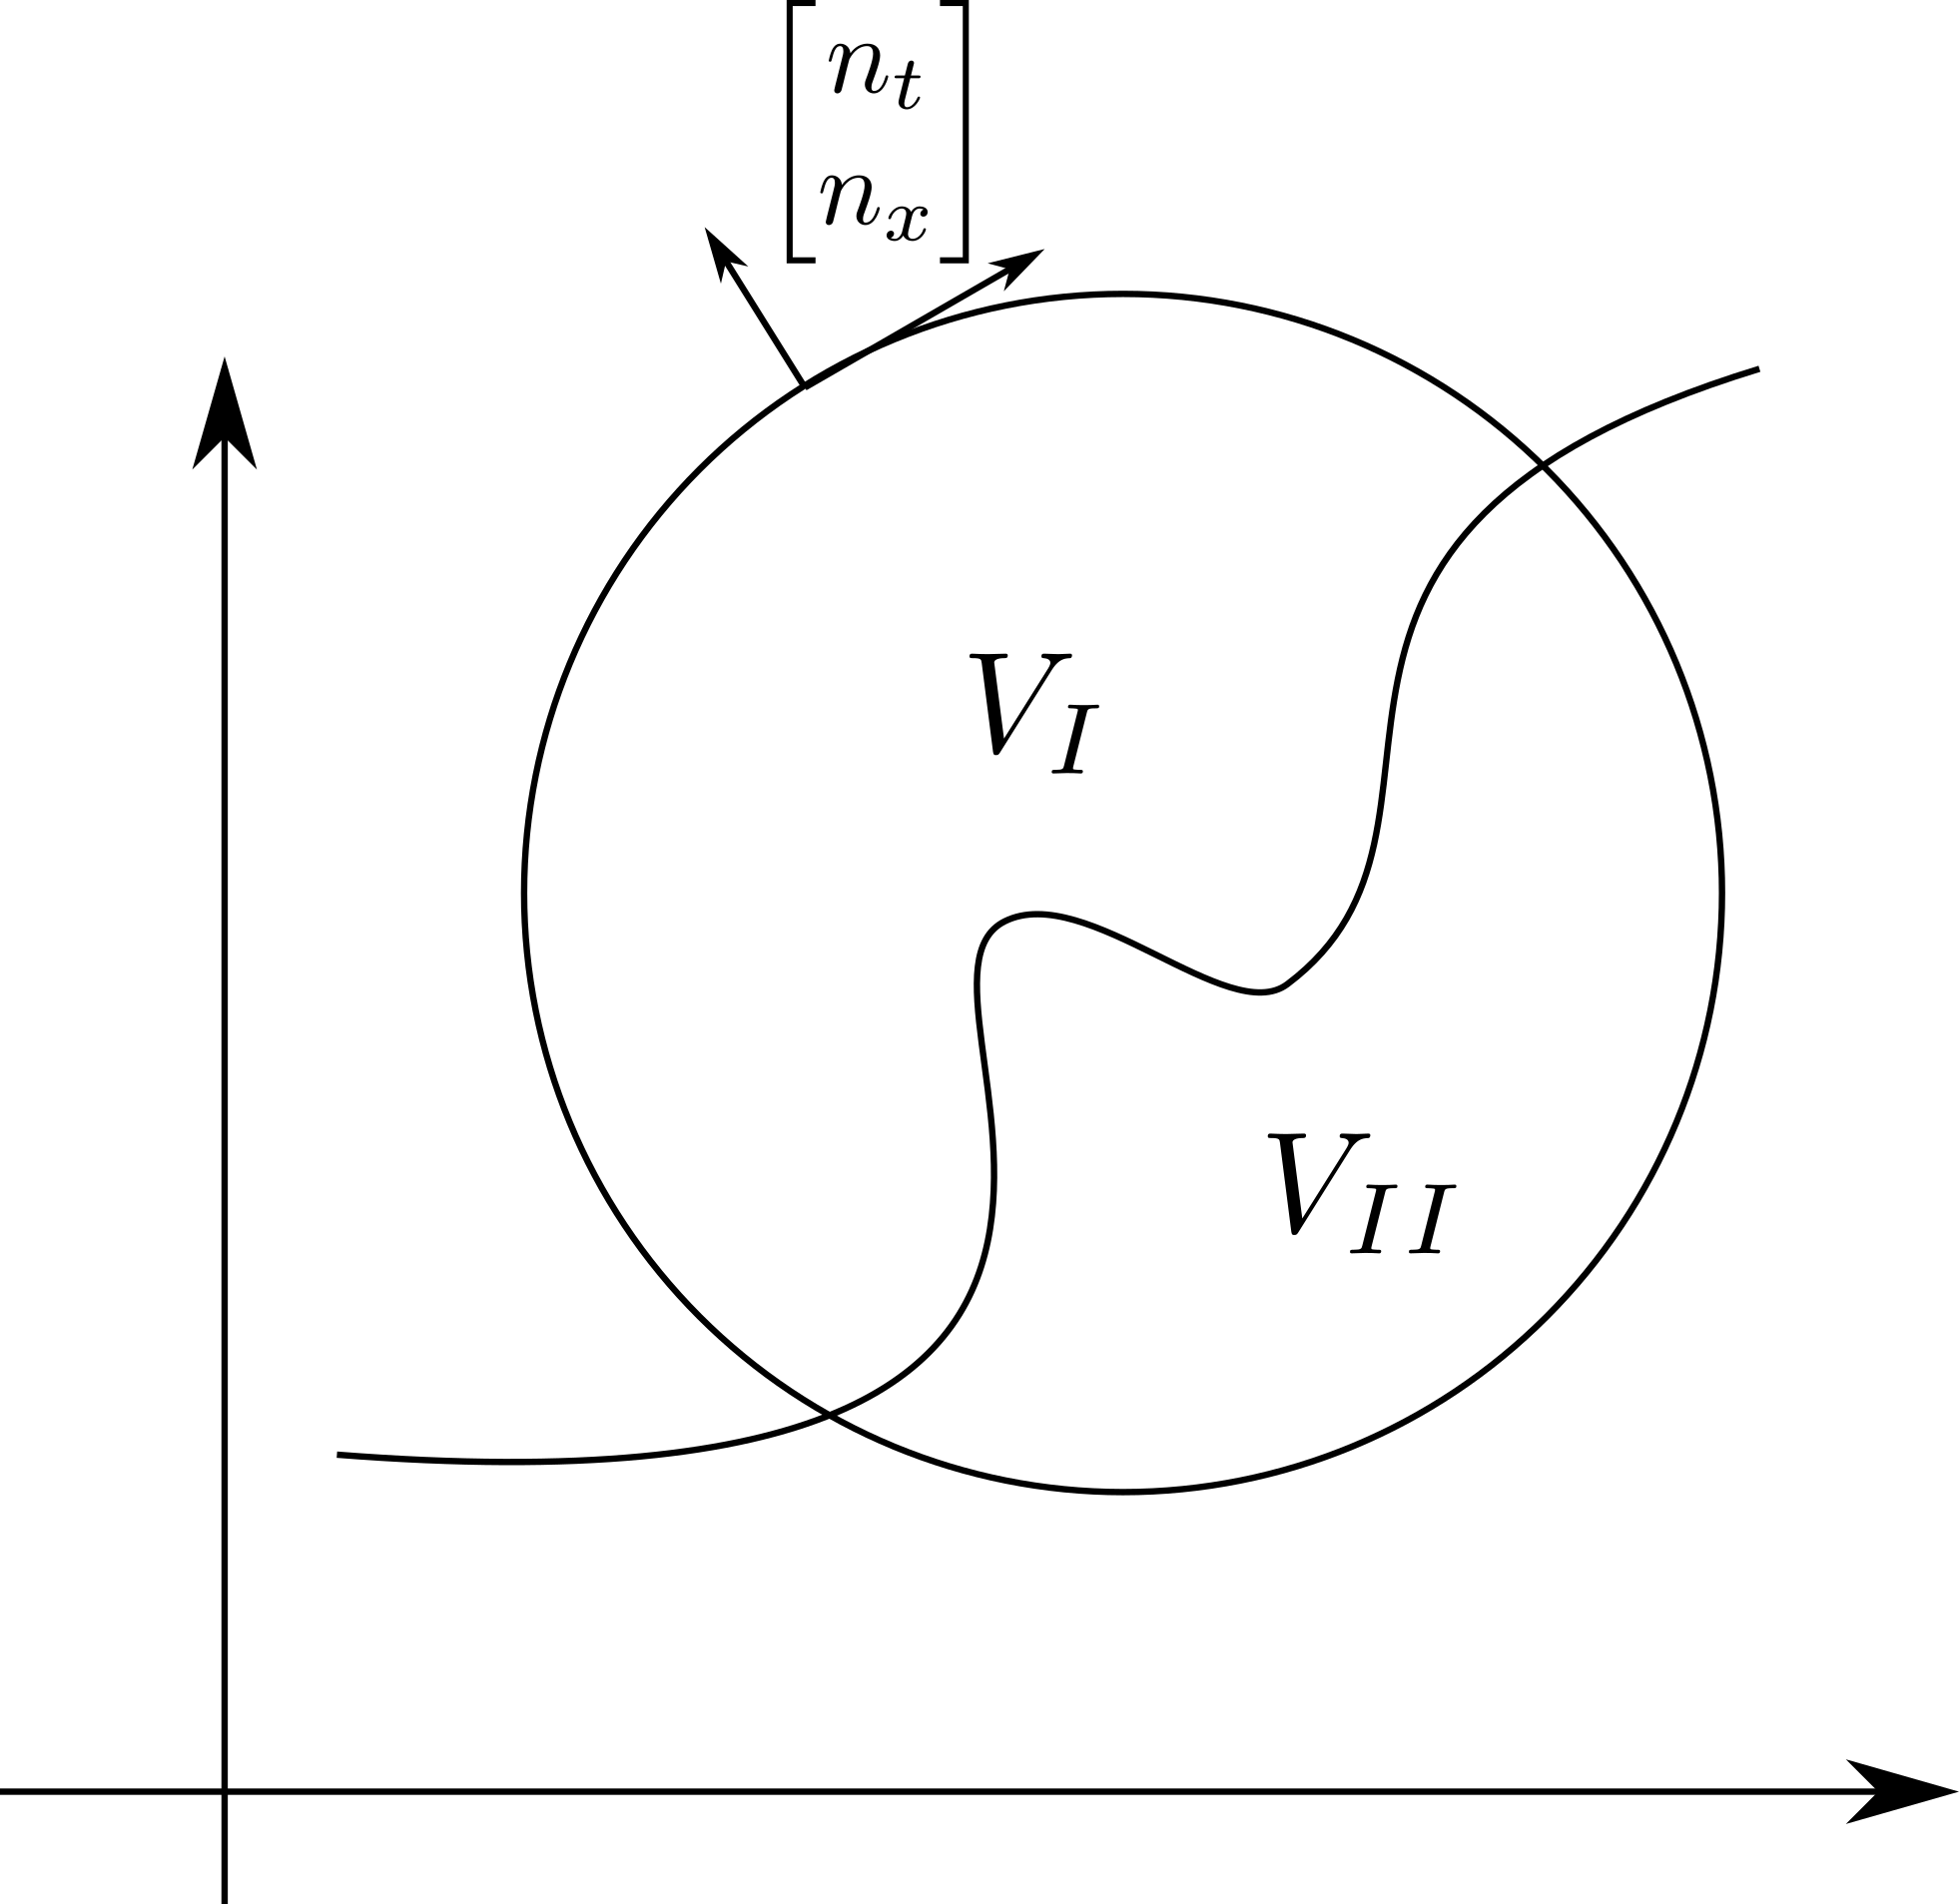
\includegraphics[width=0.4\textwidth]{podzial_przestrzeni}
     \caption{Tak dzielimy sobie nasze rozwiązania}
     \label{fig:podzial_przestrzeni}
 \end{figure}

 Jeżeli $U$ jest słabym rozwiązaniem, to znaczy, że
 \[
     \underset{\varphi}{\forall} \int dx\int dt \left( U \varphi_{,t} + F\left( U \right) \varphi_{,x} \right) = 0
 .\]
 (Zakładamy, że $V$ jest daleko od linii $t = 0$, i $\varphi$ ma nośnik zwarty). To wtedy to się równa
 \[
     \underset{\varphi}{\forall} \iint\limits_{V_1} \left( U \varphi_{t} + F(U)\varphi_{,x} \right) + \iint\limits_{V_2}\left( U \varphi_{,t} + F(U) \varphi_{,x} \right) = 0
 .\]
 Ale pierwszy człon można se scałkować przez części.
 \begin{align*}
     &\iint\limits_{V_I} U\varphi_{,t} + F(U)\varphi_{,x} = \int\limits_{V_I}dx\int\limits_{V_I}dt \left( U\varphi \right) _{,t} + \left( F(U)\varphi \right) _{,x} - \iint\limits_{V_I}dxdt\left( U_{,t} + F(U)_{,x} \right) \varphi = \\
     &= \iint\limits_{\partial V_I}\left( (U\varphi)n_t + (F(U)\varphi)n_x \right) dL + 0
 .\end{align*}
 Analogicznie
 \[
     \iint\limits_{V_{II}} U\varphi_{,t} + F(U)\varphi_{,x} = \int\limits_{\partial V_{II}}\left( U^{II}\varphi \right) n'^t  + F(U^{II})\varphi)n'^x  + 0
 .\]
 Ale \[
     \begin{bmatrix} n^t\\n^x \end{bmatrix} = -\begin{bmatrix} n'^t\\n'^x \end{bmatrix}
 ,\]
 więc warunek sprowadza się do
 \[
     \int\limits_{\partial V_I \cap \partial V_{II}} \left( (U^I - U^I)n^t + \left( F(U^I) - F(U^{II})n^x \right) \varphi \right) = 0
 .\]

 $\partial V_I \cap \partial V_{II}$ poza częścią wspólną zakładamy, że $\varphi = 0$, bo ma zwarty nośnik.

\end{document}
